\subsection{Обобщение числа соседей до случайных блужданий с самопересечениями}

В качестве завершения исследования поведения долей узлов с фиксированным числом соседей рассмотрим случай базового случайного блуждания, в которой отсутствует ограничение самопересечений. Как в предыдущих разделах, исследуемыми свойствами будет как общее поведение долей узлов с фиксированным числом соседей, так и атмосферы на концах блужданий с увеличением длины блуждания. 

Важно отметить, что в данном случае появиться дополнительная наблюдаемая - доля уникальных узлов, занимаемых блужданием. Очевидно, что в SAW-моделях число шагов блуждания и количество занимаемых узлов являются почти идентичными понятиями, особенно в бесконечно больших конформациях. В свою очередь, без ограничения на самопересечения, простое случайное блуждание будет попадать на ранее посещённые узлы, и разница между этими понятиями будет ощутима. Поэтому, для чистоты исследования, понятие "длина блуждания" будет раздвоено:

\begin{itemize}
\item Количество шагов простого случайного блужания $N$
\item Количество уникальных узлов блуждания $\Nun$ - в рамках поиска средних наблюдаемых $\la \Nun \ra = N * \la \nun \ra$ 
\end{itemize}

\begin{figure}[h]
    
\begin{minipage}{0.49\textwidth}
    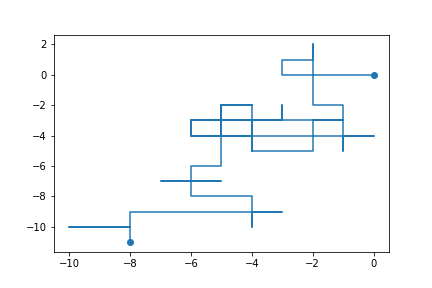
\includegraphics[width=\textwidth]{Sections/Images/Rand_Path.png}
    \caption{Пример сгенерированного блуждания Random-Walk}
    \label{fig:path_1}
\end{minipage}
\hfill
\begin{minipage}{0.49\textwidth}
    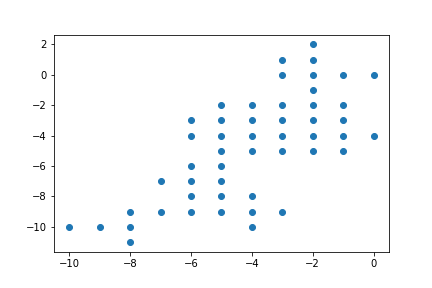
\includegraphics[width=\textwidth]{Sections/Images/Rand_Path_Unique.png}
    \caption{Набор уникальных точек, принадлежащих блужданию Random-Walk}
    \label{fig:path_2}
\end{minipage}
\centering
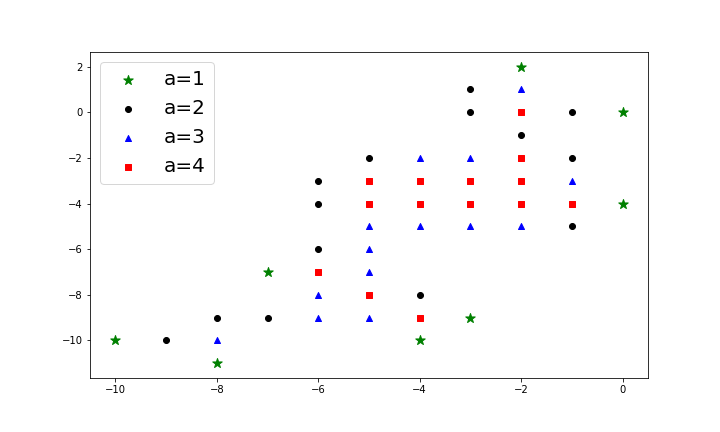
\includegraphics[width=0.5\textwidth]{Sections/Images/Rand_Path_Neigh.png}
\caption{Пример подсчёта соседей у каждого узла блуждания}
\label{fig:path_3}
\end{figure}

\subsubsection{Алгоритм генерации блужданий}

Блуждания легко генерируются в виде последовательности индексов направлений $ {a_{N}} $ в любой решётке, что ускоряет процесс моделирования. 
Тогда, начиная с некоторой начальной точки на решётке $\omega_{0}$, блуждание определяется как последовательность узлов $ 
\omega_{i} = \omega_{i-1} + steps\left[a_{i}\right] $, где $steps$ - массив фиксированных смещений из точки, определяемые законами решётки. 
Точность подсчёта наблюдаемых определяется лишь количеством повторов эксперимента.

С другой стороны, отсутствие требования правильности блуждания вызывает ряд осложнений для сравнения результатов с классом блужданий без самопересечений. 
Например, возможны случаи, когда два идущих подряд направления противоположны друг другу - то есть, на i-м шаге блуждание смещается из точки $\omega_{i-1}$, а i+1-м - возвращается в него, то есть $\omega_{i-1} = \omega_{i+1}$.
В таком случае на графике блуждания возможны ''шипы'', концы которых будут узлами с всего одним соседом - основанием ''шипа''. 



Алгоритм обработки каждого модерируемого блуждания описан на картинках \ref{fig:path_1}, \ref{fig:path_2} и \ref{fig:path_3}:
\begin{itemize}
    \item Из случайного блуждания отбираются все уникальные точки узлов
    \item Для каждого уникального узла рассчитывается кол-во его соседей 
    \item Доля узлов с k соседями считается как {количество уникальных узлов с k соседями}/{общее кол-во уникальных узлов}
\end{itemize}

\subsubsection{Результаты симуляций}

Была проведена генерация модели случайного блуждания с самопересечениями (далее Random-Walk или RW) для длин $10^{2}-10^{4}$. 
Рассматривалась доля узлов с фиксированным числом соседей - от 1 до 4 - среди уникальных узлов в итоговой конформации, для чистоты результатов и возможности сравнения с результатами случайного блуждания без самопересечений.
Доли уникальных узлов так же бралась во внимание при симуляциях. 
Результаты симуляций, а так же количество итераций для каждой длины, описаны в таблице \ref{tab:Ran_Walk_neigh} и изображены на графиках \ref{fig:DS_n_i}, \ref{fig:DS_n_iu} и \ref{fig:DS_n_u}.\footnotemark{}.\footnotetext{Процесс симуляций был запрограмирован на языке Python и проводился с использованием суперкомпьютера НИУ ВШЭ. Оптимизация требовала дополнительного изменения окружения - см. технический раздел\ref{subsection:njit_problem}}

\begin{table}[h]
    \centering

\begin{tabular}{|c|c|c|c|c|c|c|}
\hline
N & steps & $ \nun $ & $n_{1}$ & $n_{2}$ & $n_{3}$ & $n_{4}$ \\ \hline
100 & 96430000 & 0.490868(8) & 0.067676(3) & 0.33516(1) & 0.357310(7) & 0.239851(9) \\ \hline
150 & 69360000 & 0.462622(9) & 0.057825(3) & 0.30787(1) & 0.356280(7) & 0.27802(1) \\ \hline
200 & 36140000 & 0.44436(1) & 0.052236(4) & 0.29043(1) & 0.353706(9) & 0.30362(2) \\ \hline
350 & 17070000 & 0.41251(2) & 0.043761(4) & 0.26070(1) & 0.34590(1) & 0.34963(2) \\ \hline
500 & 7720000 & 0.39439(2) & 0.039590(5) & 0.24424(2) & 0.33965(2) & 0.37652(3) \\ \hline
750 & 4810000 & 0.37559(2) & 0.035672(5) & 0.22759(2) & 0.33188(2) & 0.40487(4) \\ \hline 
1000 & 2480000 & 0.36325(3) & 0.033333(6) & 0.21696(3) & 0.32610(2) & 0.42361(5) \\ \hline
3000 & 420000 & 0.32265(6) & 0.02650(1) & 0.18336(5) & 0.30351(5) & 0.4865(1) \\ \hline
5000 & 140000 & 0.30679(9) & 0.02434(1) & 0.17086(8) & 0.29322(8) & 0.5116(2) \\ \hline
6500 & 100000 & 0.2992(1) & 0.02330(2) & 0.16518(9) & 0.28816(9) & 0.5234(2) \\ \hline
7000 & 305000 & 0.29610(6) & 0.02302(1) & 0.16340(5) & 0.28657(5) & 0.5270(1) \\ \hline
8000 & 240000 & 0.29338(6) & 0.02253(1) & 0.16070(5) & 0.28409(6) & 0.5327(1) \\ \hline
9000 & 195000 & 0.29022(7) & 0.02215(1) & 0.15830(6) & 0.28185(6) & 0.5377(1) \\ \hline
10000 & 160000 & 0.28751(8) & 0.02179(1) & 0.15628(6) & 0.27991(7) & 0.5420(1) \\ \hline
\end{tabular}

    \caption{Средние доли узлов c 1-4-мя соседями в конформациях модели Random-Walk длин $10^{2}-10^{4}$. Также изображены на графиках \ref{fig:DS_n_i}, \ref{fig:DS_n_iu} и \ref{fig:DS_n_u}.}
    \label{tab:Ran_Walk_neigh}
\end{table}

\begin{figure}[h]
    
\begin{minipage}{0.49\textwidth}
\centering
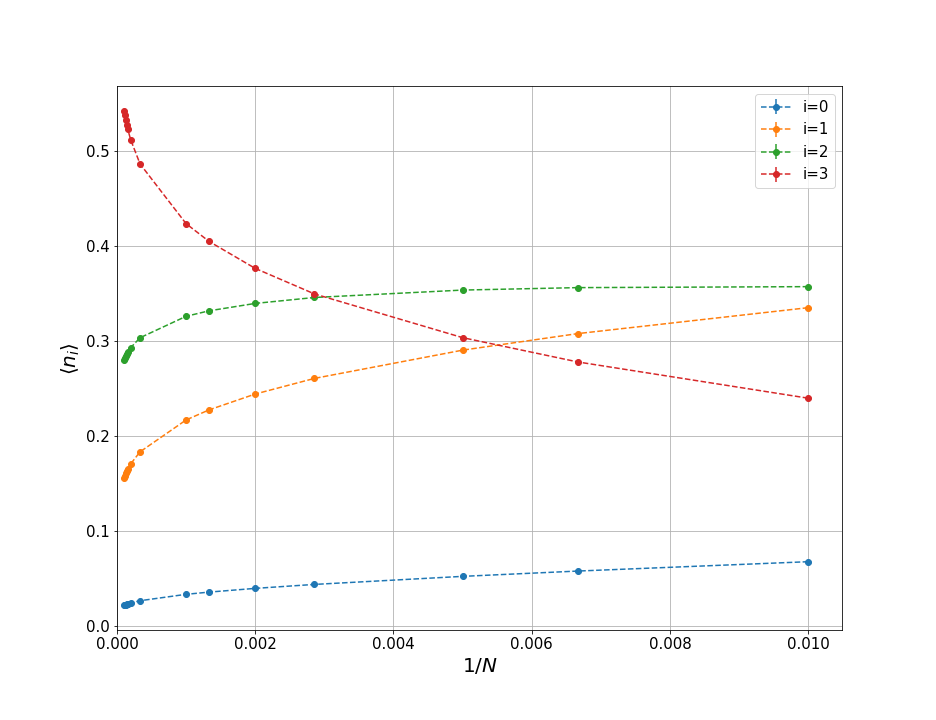
\includegraphics[width=\textwidth]{Sections/Images_2/Rand_Path_n_i.png}
\caption{Зависимость долей узлов с фиксированным числом соседей от обратного количества шагов блуждания $1/N$  (столбцы $n_{1-4}$ из таблицы \ref{tab:Ran_Walk_neigh})}
\label{fig:DS_n_i}
\end{minipage}
\hfill
\begin{minipage}{0.49\textwidth}
\centering
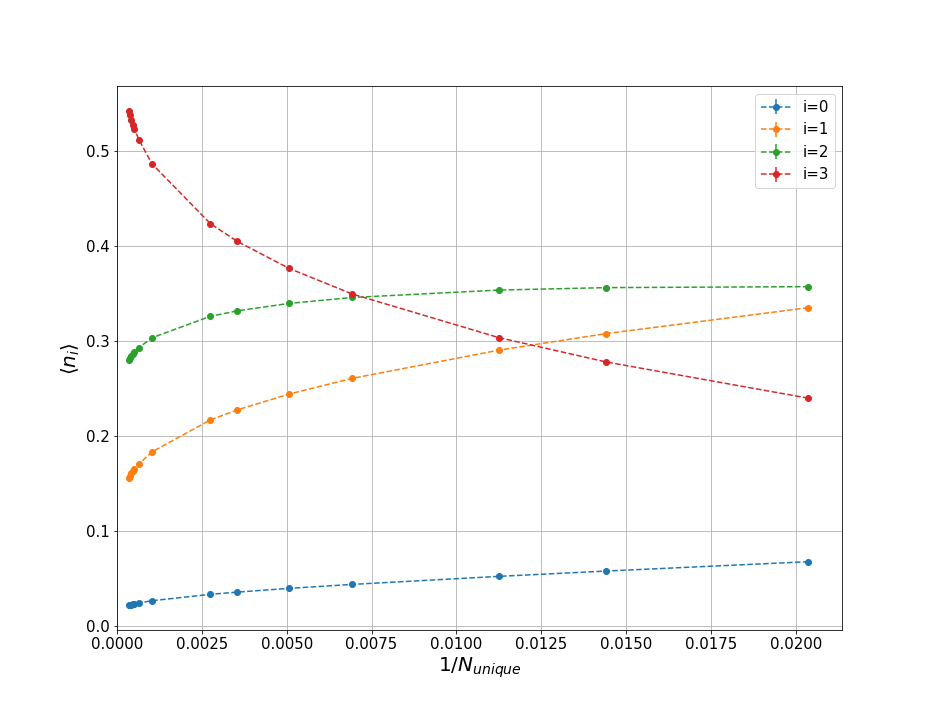
\includegraphics[width=\textwidth]{Sections/Images_2/Rand_Path_n_i_unique.png}
\caption{Зависимость долей узлов с фиксированным числом соседей от обратного количества уникальных узлов $1/\Nun$  (столбец $n_{1-4}$ при длине блужданий $N * \textup{unique}$ из таблицы \ref{tab:Ran_Walk_neigh})}
\label{fig:DS_n_iu}
\end{minipage}
\centering
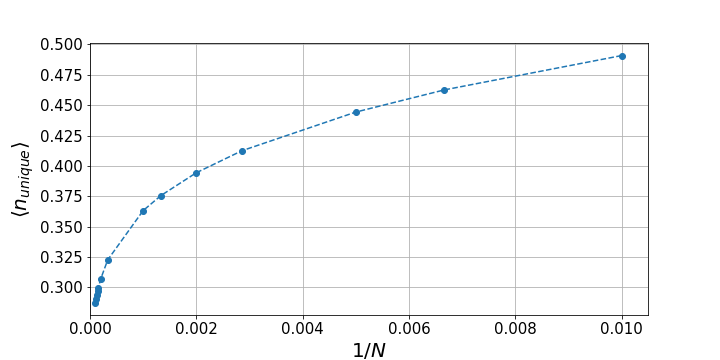
\includegraphics[width=0.6\textwidth]{Sections/Images_2/Rand_Path_n_unique.png}
\caption{Зависимость долей уникальных узлов от обратного количества шагов блуждания $1/N$ (столбец $\nun$ из таблицы \ref{tab:Ran_Walk_neigh})}
\label{fig:DS_n_u}
\end{figure} 

\newpage

\subsubsection{Погрешности результатов}

Полученные в данной подсекции результаты имели ранее необоснованно большие погрешности, что потребовало более тщательного исследования. 
Необходимо проверить распределение результатов со временем, а так же сходимость средних наблюдаёмых величин и их ошибок.
 В качестве примера рассмотрим первую исследуемую длину $N=100$, т.к. именно её симуляции протекают быстрее всех.  

Распределение наблюдаемых долей узлов с фиксированным числом соседей 1-4, а так же доли уникальных узлов рассмотрены на гистограммах на левом графике рисунка \ref{fig:DS_100_dists_history}  в двух моментах времени: после $10^6$ шагов и после $2.5 * 10^6$  шагов. 
На рисунке видно, что данные всех величин имеют нормальное или близко к нормальному распределению, а несимметричные склоны  некоторых величин ($n_1$ и $n_2$) объясняются близостью соответствующего края к нулю.

Сходимость наблюдаемых величин можно увидеть на правом графике \ref{fig:DS_100_dists_history}, где замеры средних проводились через каждые 4000 шагов. На графике средних заметна сходимость средней величины и уменьшение колебаний. 
С другой стороны, график среднего квадратического отклонения не стремится к нулю как ожидалось, а так же сходится с уменьшением колебаний к ненулевому значению. 
Это показывает противоречивость результатов (по крайней мере замеров ошибки - среднее явно сходится), причину чему следует искать в коде. 

Для удостоверения, что причина не лежит в jit-компиляции, был проведён запуск нескомпилированного с помощью numba кода. Результаты оказались идендичны с jit-компиляцией, и следовательно проблема в другом месте.

\begin{figure}
	\caption{Слева: Распределение долей узлов с 1-4 соседями и уникальных узлов блуждания длины 100 в два момента времени. Справа: История результатов (Столбец mean - средняя величина, столбец std - значение ошибки на i-м замере) долей узлов с 1-4 соседями и уникальных узлов блуждания длины 100 с интервалом замеров в 4000 шагов}
     \label{fig:DS_100_dists_history}
\begin{minipage}{0.32\textwidth}
     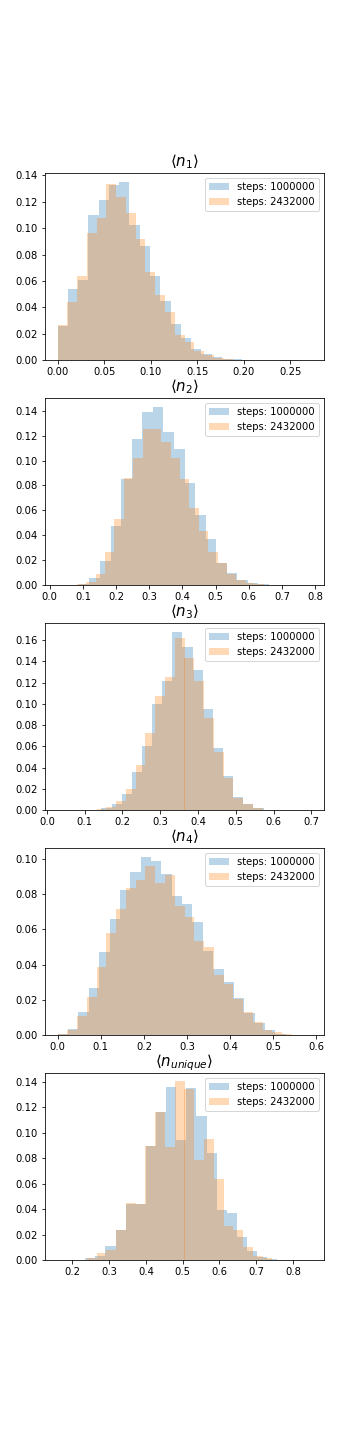
\includegraphics[width=\textwidth]{Sections/Images_2/DS_100_dists.png}
\end{minipage}
\begin{minipage}{0.67\textwidth}
     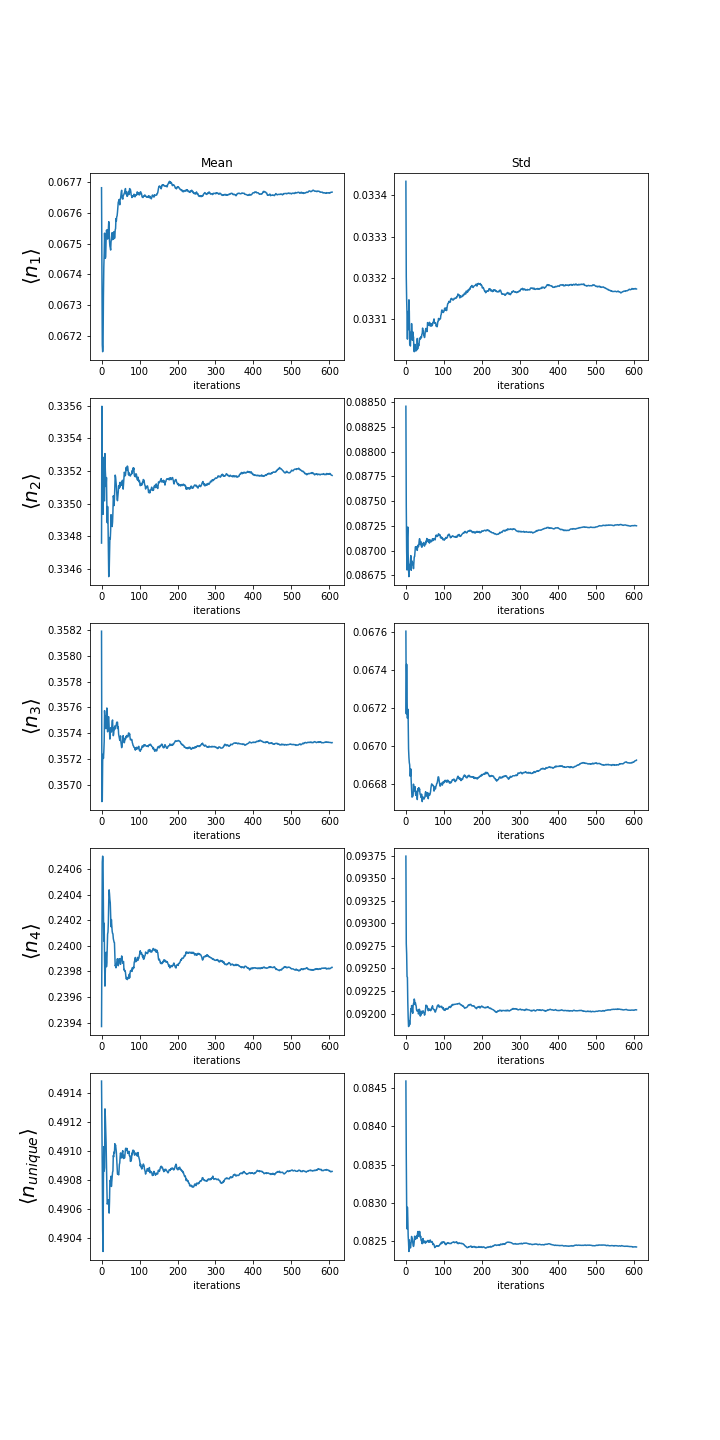
\includegraphics[width=\textwidth]{Sections/Images_2/DS_100_history.png}
\end{minipage}
	
\end{figure}


Причиной столь больших погрешностей результатов была неверная интерпретация понятия "ошибка среднего", толковавшаяся ранее, как выборочное среднее квадратическое отклонение $\sigma(x)$ результатов симуляций $x$ - на деле ошибкой среднего является формула вида:

\[\Delta\la x \ra = \sigma(x)/\sqrt{N},\]

где  $N$ - объём выборки или количество экспериментов.


\subsubsection{Шкалирование результатов и его графические особенности}

Применим к результатам вероятности атмосфер те же методы анализа на бесконечности, что и ранее для доли узлов с фиксированным числом соседей в СБС - определим характер шкалирования значений вероятности при стремлении длины конформации блуждания rand\_walk к бесконечности.
Рассмотрим данные в трёх предполагаемых масштабах: в линейной, лог-линейной и лог-логарифмической масштабностях от обратной длины $1/N$ и кол-ва уникальных узлов $1/\Nun$.
Пример исследуемых данных показан на графике \ref{fig:n1_scale}. 
На нём видно, что в случае лог-лог-шкалирования (или степенного) график обретает наилучшую среди трёх масштабностей линейность.
Аналогичное наиблоее подходящее шкалирование показали графики всех долей узлов $n_{1-4}$ в зависимости от обоих длин блуждания, а так же $n_{unique}$ от кол-ва шагов $N$.

\begin{figure}
\centering
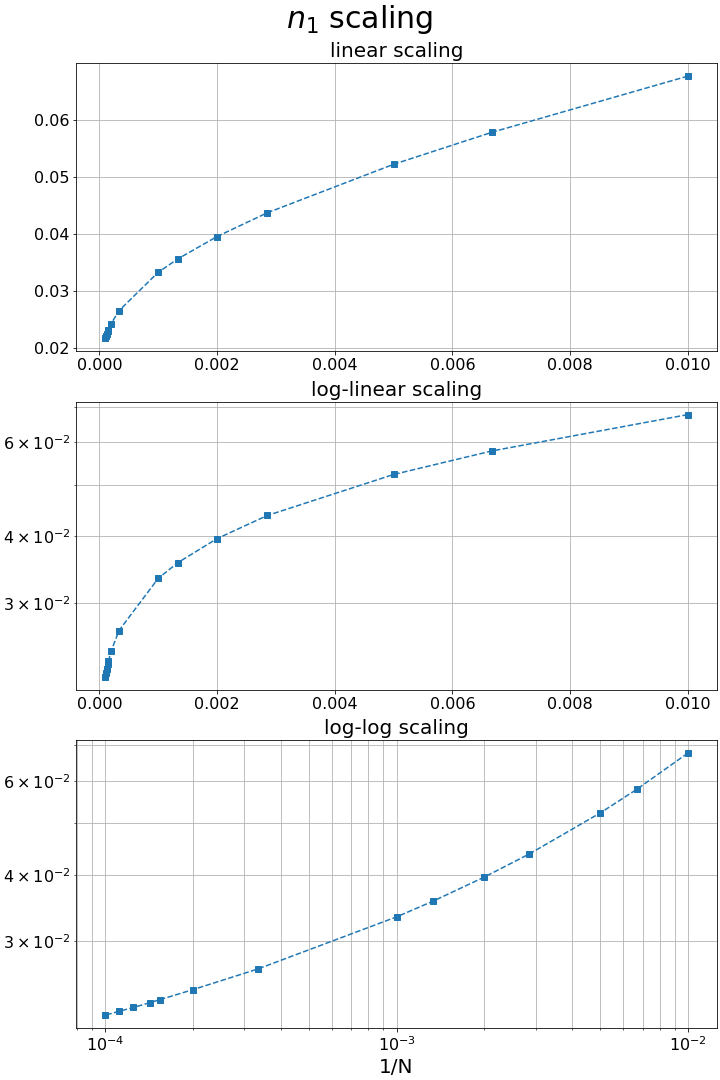
\includegraphics[width=0.7\textwidth]{Sections/Images_2/n1_res.png}
\caption{Зависимость $n_1$ от $1/N$  в линейной, лог-линейной и лог-логарифмической масштабностях (сверху-вниз), по данным из таблицы \ref{tab:Ran_Walk_neigh}} 
\label{fig:n1_scale}
\end{figure}

Тогда, предполагаемая фитирующая функция рассматривается двумя способами: в первом случае - как зависимость доли уникальных узлов с фиксированным числом соседей, а так же доли уникальных узлов блуждания, от количества шагов $N$:

\begin{equation}
\la n_{i} \ra (N) = k_i * (1/N)^{a_i} + b_i,\ \ \ i \in \{1,2,3,4, \textup{unique}\}
\label{eq:n_i_log_log}
\end{equation}

Полученные коэффициенты с погрешностями выписаны на таблице \ref{tab:n_i_log_log}.

\begin{table}[h]
\centering
\begin{tabular}{|c|c|c|c|c|}
\hline
 & k & a & b & N \\ \hline
$n_1$ & 0.3425(8) & 0.417(2) & 0.014(1) & 3000-10000 \\ \hline
$n_2$ & 0.573(4) & 0.171(1) & 0.037(2) & 3000-10000 \\ \hline
$n_3$ & 0.588(3) & 0.219(3) & 0.202(3) & 3000-10000 \\ \hline
$n_4$ & -1.239(9) & 0.189(3) & 0.759(5) & 500-10000 \\ \hline
$n_{unique}$ & 0.831(1) & 0.2049(2) & 0.1616(4) & 500-10000 \\ \hline
\end{tabular}
\caption{Коэффициенты степенной фитирующей функции доли узлов от обратного количества шагов блуждания $1/N$ \ref{eq:n_i_log_log}}
\label{tab:n_i_log_log}

Аналогичный анализ проведён для зависимости долей узлов $n_1 - n_4$ от количества уникальных узлов $\Nun$:

\begin{equation}
\la n_{i} \ra (\Nun) = k_i * (1/\Nun)^{a_i} + b_i,\ \ \ i \in \{1,2,3,4\}
\label{eq:n_i_u_log_log}
\end{equation}

\begin{tabular}{|c|c|c|c|c|}
\hline
 & k & a & b & $\Nun$ \\ \hline
$n_1$ & 0.313(1) & 0.479(2) & 0.015(1) & 967-2875 \\ \hline
$n_2$ & 0.567(3) & 0.214(1) & 0.053(2) & 967-2875 \\ \hline
$n_3$  & 0.542(5) & 0.244(2) & 0.203(2) & 967-2875 \\ \hline
$n_4$ & -1.20(1) & 0.225(4) & 0.741(5) & 197-2875 \\ \hline
\end{tabular} 
\caption{Коэффициенты степенной фитирующей функции доли узлов от обратного количества уникальных узлов блуждания $1/N_{unique}$ \ref{eq:n_i_u_log_log}}
\label{tab:n_i_u_log_log}
\end{table}

Поравное сравнение соответствующих коэффициентов функций между таблицами \ref{eq:n_i_u_log_log} и \ref{tab:n_i_u_log_log} не даёт точного ответа, есть ли какая-либо связь между значениями коээфициентов функций от разных "длин": 
между данными существует лишь два пересечения значений в пределах погрешностей: коэффициент $k_2$, $b_1$ и $b_3$. 
В целом столбцы коэффициентов $k$ и $b$ похожи между таблицами и с точностью до первого знака после запятой (что на несколько порядков больше имееющейся погрешности) равны. Так же функции имеют иденчичное знаковое поведение между аргументами (что видно по коэффициенту $k_4$).
Однако более глубокого численного сходства между функциями не наблюдается.
Это можно объяснить в графическом сравнении между общими графиками \ref{fig:DS_n_i} и \ref{fig:DS_n_iu} - во втором случае график расстягивается вправо, причём, как видно из значений долей уникальных узлов от количества шагов \ref{fig:DS_n_u}, с ростом N смещение становится сильнее (от 2 раз справа до более чем 3 раз слева).


\newpage 